\chapter{Mysore District Environment}

Assemblage of birds found in any region is governed by 
environmental conditions stretching across the territory. The 
topography, climate and type of vegetation which is directly or 
indirectly influenced by climate give rise to varied habitats in 
the environment. Their conditions are further modified by seasonal 
changes which trigger various natural phenomenon like flowering, 
winter leaf-fall, bursting forth of new leaves, breeding 
activity, migration, emergence of insects, and abundance of 
birds. An overview of the part of the region that constitutes 
Mysore District will give us a broad perspective against which 
the bird life can be observed. It will also help in understanding 
ecological relations of the birds. 

Even within the natural settings human pressure is increasing 
and the landscape is undergoing slow and gradual change. Some 
of the original landscapes which constituted well wooded areas a 
few centuries back have all but vanished. The earlier reports 
mentioned about the most magnificent forests that existed around 
Begur \& Kakankot. The forests in these areas have been over exploited 
for teak and rosewood. 

In some places the forests stand as vestiges at the edge of 
man made environment. In places forests have shrunk giving rise 
to newer landscapes called scrub with stunted trees intermingled 
with thorny thickets. The afforested areas with newer species 
have created totally different conditions in the protected areas. 
Return to the natural flora may be taking place gradually. Incidentally 
the birds have not totally shied away from these newer 
environments. However the species composition will not be the 
same and change according to availability of food, cover, and 
availability of breeding places. Many have taken refuge in parks 
and gardens in urban areas which more or less present woodland 
scenarios. 

Geographically Mysore district (coordinates 11$^\circ$.36 13$^\circ$.35 
North, 75$^\circ$.55$-$77$^\circ$.20 East) is situated at the southern tip of 
Deccan Plateau. The southern plateau stretches from the foothills 
of the Western Ghats to the broken chain of Eastern Ghats with 
average elevation of 800 mt, and covers an area of 16.00 KM$^2$. It 
is an elevated table land broken up by rocky hills and scored by 
deep ravines and extends upto foothills of Nilgiri in south. On 
the Southern side we find Gopalaswamy Hills while Billigirirangan 
hills stretch on South eastern side. Malai Mahadeshwara Hills 
extends towards Eastern Ghats. 

The area between the hill region is a rolling plain, called 
in Kannada Bayalusime. The river Cauvery flows across the eastern 
side of the district and the Southern border is delimited by 
Moyar river which courses through the thickly wooded jungles. The 
river Kabini drains northwards across the Southern Plateau and 
joins Cauvery at T.Narsipur. 

The forest belt runs through West Hunsur Taluk and spreads 
into Southern region around the hill ranges which include the 
famous Nagarhole and Bandipur. Very dense tropical forests surround 
the extreme south along the Moyar river. In the Southwest 
region the semi-evergreen and deciduous forests give way to 
scrub jungles. Such jungles are seen on the lower elevation of 
Chamundi Hills, Yelwal, area surrounding Sargur, Arekankadu (on 
way to Bandipur) and at the foot of major hill ranges. 

The further degradation of the scrub jungles is seen in 
areas close to human habitation where these regions are converted 
into barren landscapes (28\%). The total forested area in Southern 
part of the district is 1,18,220 hectare, which is above 5\% of 
the total geographical area. About 48\% of land lying in lower 
elevation is cultivated. The central portion of the district is 
intensively farmed. The Irrigation channels run through this 
portion. There are a large number of shallow irrigational tanks. 
The total water spread including reservoirs is 29,800 hectares. 
The wetlands including reservoirs, tanks, rivers, irrigational 
channels are about 1\% of the total area. 

\chapter{Natural Vegetation}

The vegetation forms major habitats. The habitats and their 
sub-divisions will ultimately form specific niches. Birds show 
fine adaptations to the niche. Niche could be considered as a 
kind of address of the bird. 

In the Mysore District we may differentiate vegetation in 
three major types. 
\begin{enumerate}
\itemsep=2pt
\item Moist Deciduous Forests 

\item Dry Deciduous Forests 

\item Thorn Scrub Forests 
\end{enumerate} 

\underline{Moist Deciduous Forests} are seen between Kakanakote and
Kerala borders, higher slopes of B.R. Hills and M.M. Hills. Tree 
layers are with open canopy. In this area the timber trees like 
Nandi, Teak, Matti are dominant. Thick climbers and epiphytic 
orchids dot some trees. Due to open canopy shrub layer grows 
underneath and is made up predominantly by Bodin gida and Kodasize. 

\underline{Dry Deciduous Forests} are adapted to long dry period. The 
trees are shorter and often protected by thorns and prickles. 
Thorny thickets form undergrowth. Climbers are wiry and often 
with latex. Xerophytes are not uncommon. Dinduga, Alule and 
Taremara form principle broad leaved trees. The forest looks 
resplendent with yellow flowers of Arsina, burges during dry 
months. Such areas are found in the forests of Nagarhole, Bandipur, 
Nugu and lower parts of B.R. Hills. 

\underline{Thorn Scrub Forests} : As trees within the woodlands are turned 
into wood Savannah landscape, with further degradations only isolated 
thickets dot the country side ultimately giving way to 
scrub. These stages are seen between Gundalpet and Gopalaswamy 
Betta. Thorny scrub type plant cover is usually found in low 
rainfall areas. The trees are slow growing, twisted and stunted, 
and armed. The hardy species like Ane, Gobli, Kudussage, Chigare 
are found here. Shrubs are wiry and thorny, and form impenetrable 
undergrowth. This is very well seen in Chikkanhalli forest and 
along Chamundi Hills. 

Besides these principle vegetation and divisions, sholas are 
found in B.R. Hills at 1400--1800 m. Along the principle river 
are seen the typical riverine forests. In the innumerable wetlands 
are seen water plants like nymphaea, nelumbo, aaponogeton, 
potamogeton and submerged plants like hydrilla, hydrophylla and 
other pond weeds. Many water bodies are covered with water hyacinth. 
The emergents like bulrushes and phragmites border along 
the marshes. These can be seen along the shallow regions in 
Kukarahallikere, Dadahalli, Mugunhundikere. 

A large number of trees are planted in open fields on the 
borders of arable lands, in village topes and along roadside. Besides 
large tracts of barren wasteland and hilly areas have been 
afforested with mainly eucalyptus species. One can even see a 
regenerated forest at Chikkanahalli near Mysore. This background 
will serve as a framework for understanding ecological relationship 
of birds. It is a virgin field and every bird watcher can 
contribute towards the knowledge of bird ecology. One can also 
enhance the pleasure of bird watching by sharing his experience 
with others. 

\chapter{Distribution of birds in the region}

The humid hills of Kerala, Wynad, part of Mysore, Bandipur, 
Nagarahole, Madhumalai form a contiguous sub region of Western 
Ghats. The bird life in this area is very characteristic and 
resembles species which occur in the North East India and Burma. 
Besides climate and availability of food, the other factors like 
height of the trees, open or closed canopy, secondary growth 
nesting material, open spaces and roads are important factors in 
the distribution of birds. The broad leaves of trees in the dry 
deciduous forest provide habitats for large number of birds. 
Hence highest number of species are recorded in dry deciduous 
forest. Similarly large number of species are found where man has 
altered the landscape by selection of trees species and the 
distribution of the trees. It is usually mixed with natural 
growth. This gives rise to variety of covers in parks, campuses, 
gardens. The diversity of environment is artificially high and it 
attracts large number of birds. In degraded forests the number of 
species gradually diminish. In open country and agricultural 
lands the number of birds is usually sparse. Most birds come for 
foraging. On the other hand in wetlands the avifuana depends on 
richness and diversity of micro habitats. 

The list of birds found in the major habitats is appended. 
The list will serve as guidance. There may be many important 
omissions and the list can be augmented by sharing information 
with other bird watchers. Some birds will be common to all 
habitats. Many times birds from adjacent area are also listed. Some birds 
are equally restricted to specific habitats. There is a lot of 
overlap seen as in nature, there are no clear cut demarcations or 
zones. Not all birds seen are found frequently. One will be able 
to make new discoveries in the course of his observations. All 
this makes bird watching an exciting hobby. 

\thispagestyle{empty}

\vbox to\textheight{\vfill\hbox to\textwidth{\hfill\rotatebox{90}{\includegraphics{map/map.jpg}}\hfill}\vfill}

\addtocontents{toc}{\protect\contentsline{chapter}{4~~~ \protect Map of Mysore District - Physical Feature}{\thepage}}

\setcounter{chapter}{4}

\chapter{A B C of Bird Watching}%%%4

Bird watching as an activity could be carried out for sheer 
pleasure of observing birds in their environment. After sometime 
it may become a serious study of exploring Nature. Whether it is 
pursued as a hobby or as a scientific interest, bird watching 
needs to be done in a systematic manner. 
\begin{enumerate}
\itemsep=0pt
\item \underline{Before you start} : Try to get familiar with the geography of 
the area. Within 100 km you may come across different types 
of environment. It may be countryside, woodlands, forests, 
wetlands, plantations, etc.,. The birds association differ 
in different environment. They can very well be observed in 
parks, gardens and campuses. 

\item \underline{When to start} : As a beginner it is better to start when 
birds could be seen in large numbers. October to April is 
the best period. A number of migratory birds descend down to 
feed in marshes and wetlands. 

The birds are active during early morning or before 
dusk. The timings for bird watching : 
\vskip 2pt

\centerline{\begin{tabular}{ccc}
7 a.m. & to & 10 a.m. \\
& \& & \\
4 p.m. & to & 6 p.m.
\end{tabular}}
\smallskip

\item \underline{What we need} :
\begin{itemize}
\item[(i)] Dress : Dull Green or Brown coloured. The dress should 
blend with surrounding. Black, white or striking coloured 
dresses should be avoided. 

\item[(ii)] Rubber soled shoes. 

\item[(iii)] A cap 

\item[(iv)] Binocular size 8 $\ast$ 30 (8 - magnification, 30 - diameter 
of object lens in mm.) 

\item[(v)] A field notebook. 

\item[(vi)] A hand guide on birds. There are a few other things one 
need when carrying out studies like maps, camera, tape 
recorder, etc.,. The beginner should not worry about 
them. 
\end{itemize}

\item \underline{How to observe} :
\begin{itemize}
\item[(i)] Make full use of eyes and ears. They are equally important 
tools. It is better to get familiar with bird calls. 

\item[(ii)] Choose a place from which one may be able to scan a 
large area, e.g. sitting on a mound, under a large 
shady tree. 

\item[(iii)] Always walk zigzag, circular or alongside of the bird. Do 
not approach the bird directly. 

\item[(iv)] Use binocular for details. Do not observe constantly to 
avoid eye strain. 
\end{itemize}

\item \underline{What to observe} : Keep careful notes of all that you observe. 
It is better to get familiar with birds from their 
pictures or observing them in zoo or museum from time to 
time. 
\begin{itemize}
\item[(i)] Note down date, time, weather, locality. 

\item[(ii)] Size  : Sparrow, bulbul, myna, crow or kite 
(bigger - smaller). 

\item[(iii)] Shape : Slim, stout. 

\item[(iv)] Bill - Straight, pointed, curved, slender, thick, 
hooked, conical. Also note colour of the beak.

\item[(v)] Legs : Size long or short toes. 

\item[(vi)] Tail : Long, short, forked, Tip round, pointed. Also 
observe movements of tail. 

\item[(vii)] Crest over the head, colour, shape. 

\item[(viii)] Colour of body - Bright, sober. 

Colour of upper part and lower part of wings. Conspicuous 
marks, look at breast spotted, streaked, or stripped 
tail. Bands at tip. Any spots, rump. Any patch. 
In waterbirds marking on wings are important. In some 
Male and Female differ in colour and appearance. During 
breeding some birds assume breeding plumage. 

\item[(ix)] Voice : Musical, metallic, harsh, soft, trilling. 

\item[(x)] Behaviour : How birds feed and manner of eating. Behaviour 
during breeding season. Flying habit. 

\item[(xi)] Where the bird was found, on the tree, ground, on post, in 
bush, grass. 

\item[(xii)] Details about place visited: Marsh, Garden, Grove, 
Kere, Cultivated field, Fallow land, Plantation, Forest, 
Scrub. 
\end{itemize}

\item \underline{Code of Behavior} : 
\begin{itemize}
\item[(i)] Permission to enter private lands must be taken. 

\item[(ii)] While walking in cultivated lands, keep to paths. 

\item[(iii)] Don't throw away litter. 

\item[(iv)] Be careful during dry periods. By chance a match stick 
thrown on grass may start a devastating fire. 

\item[(v)] Don't disturb any natural thing. Don't touch nest, eggs, 
etc.,.

\item[(vi)] Be familiar with the Wildlife Protection Act. 
\end{itemize}
\end{enumerate}

Useful Books for Bird watchers. 
\begin{enumerate}
\item The Book of Indian Birds - by Salim Ali. 

\item Collins Hand guide to the Birds of the Indian Sub continent - by Martin Woodcock. 

\item About Indian Birds. 

Laeeq Futehally And Salim Ali 
\end{enumerate}

\chapter{Bird Watching in C.F.T.R.I Campus}

With natural habitats disappearing in countrysides, gardens and parks 
are becoming refuge for many woodland species of birds. The gardens and 
the parks in the city are small islands of woods. C.F.T.R.I campus is a sort of 
mix of garden and park where birds have been found in fairly large numbers. 
In such an environment one can almost come in contact with nature 
everyday and experience the joy of self - discovery. 

The mansion, built in Baroque style and looking resplendent in yellow 
ochre, stands at the highest elevation of the landscape. The ledges of the 
mansion provide roosting and nesting places for the feral Blue Rock Pigeons 
which are found hovering around it with their deep gootr-goo, gootr-goo 
notes. The roads leading to various blocks and residences loop around this 
stately building. It is surrounded by 100 acres of land, which is left 
untouched and it provides plenty of cover to the avian neighbours. The 
cultivated garden in the front together with the built area occupies 
comparatively a small portion of the total ground. Within last 25 to 30 years 
of its occupation by the premiere laboratory, a large area was left 
unexploited giving rise to natural growth of vegetation. To this varied 
landscape is added the rambling hedgerows and private gardens interspersed 
with buildings and thickets. Such growth is an open invitation to a large 
number of insect species like grasshoppers, crickets and other gramnivorous 
insects. The soil is perennially covered by the grasses which grow 
luxuriantly. The leaf fall from the deciduous trees during winter, and 
aftermath of cut and dried grasses, provide rich food for fungi and ants and 
many other insects which can be seen swarming all around. The leaf litter 
found under the trees and hedges shelter a large number of bugs and beetles. 
The moths though not butterflies, deposit their eggs among the succulent 
leaves with multicolored caterpillars among the garden plants. With such 
plethora of insect life there is an abundance of food, especially for the 
passerine birds. 

Since the estate was handed over to house CFTRI in 1952, lot of 
changes have taken place; the built area has increased. A mixture of natural 
and cultivated trees have occupied the campus, that is sprawling over hundred 
acres of land. A lot of shrubbery is growing along the rows of residential 
areas and the area is parceled out into boulevards, orchards and lawns. This 
man made mosaic invites a large number of woodland birds in and out of 
season. The whole campus acts like a supermarket for bird population in 
the environment of Mysore city. 

\medskip
\heading{Bird Life}
While entering through the main gate you may witness the antics of 
the Roller or Blue Jay, with brilliant display of blue bands in flight. It is a 
beauteous bird and chosen as the Bird of Karnataka. It feasts on insects, 
pouncing on them from a vantage point. Because of its blue throat it is 
considered as incarnation of Shiva. A little further, on way to the main 
building, a group of snow white little Egrets with black spear like bill will be 
seen stealthily advancing to pick up insects from the well watered lawns. 
During early periods, their lacy plumes were in great demand by milliners 
for adorning woman's hats in Europe and America. They were slaughtered 
ruthlessly almost to extinction. Luckily change in woman's fashion has 
saved them from complete extermination. A funny Spotted Owlet may be 
seen staring at you from the hollow of the large peepal tree. The ledges of 
the building provide a sanctuary for hundreds of Blue Rock Pigeons. The 
Swifts too have found a refuge there. The pigeons are seen whirling round 
the building only to return hurriedly to their perch. On way to the Southern 
gate, concealed in the leafy branches of the groves of copper pods, will be 
noticed a lonely hawk, called Shikra, lying in wait for its prey which include 
young ones of birds. 

Along the culvert, on way to school, lurks the white breasted 
Water hen. It harbours along the marshy area with its family. Among the 
thickets bordering the nullah and a patch of woodland behind the bungalows, 
I have hardly noticed any birds. Most of the varieties of birds I have noted 
are amongst the residential area behind the main building. Here, small 
flocks of crows are found. They are not the familiar House Crows with grey 
neck, but glossy jet black Jungle Crows. This is very intriguing indeed. 
Again, they have out competed the common House Sparrow from the human 
dwellings. Here and there, on open grounds, Myna's are seen loitering and 
noisily hopping. In the spring the area reverberates with kuoo-kuoo, the call 
of the male Koel. It starts with a low call reaching crescendo and breaks 
abruptly; it starts all over again monotonously. It is almost enchanting music 
heard at the break of the day from spring to pre-monsoon showers. Large 
flocks of Rose ringed Parakeets, using campus as stopover, zoom across 
screaming noisily, keeak, keeak, keeack. The Pond Heron wearing its 
maroon breeding coat, and found singly, is watching patiently for its 
favourite quarry --- the frogs. From nearby tall copper pods, we hear 
Kutroo - Kutroo, the call of the Crimson Barbet which is often mistaken for 
woodpecker. In the bushes and the hedgerows are the flower peckers and 
warblers. Warblers are busily searching for insect larvae, constantly cocking 
their slender tail and uttering tee tee from time to time. Around the 
residential quarters, you find many other birds such as Hoopoes flashing 
their hood, Minivets, with their beautiful scarlet colouring, and Common 
Brown Babblers rummaging through the litters on the ground searching for 
their prey. We are greeted by the joyful calls of the celebrated songster, the 
Redvented Bulbul. The Crested Sepoy Bulbul makes its frequent 
appearance. Bulbuls are fond of gardens. If you are lucky you may notice a 
pair of Golden Orioles among leafy trees. The Green Bee -eaters line 
themselves on over-head wires, often seen hacking their prey or gliding back 
to their base. The Crow Pheasant are heard making deep resonant call, 
coop-coop-coop, repeated quickly. They are closely related to cuckoos, and 
are considered auspicious if one comes across them. The Spotted Dove 
enters your residence and nests in the verandah in some nook. Its calls krookruk-
krukroo ... kroo-kroo - kroo, are often heard over long distances. 

One hears cheerful towit towit notes of the Tailor bird among the 
shrubs and bushy trees. One of the best songsters is the Magpie Robbin. 
Mornings are filled with its sweet songs. During breeding season, you may 
hear its plaintive notes. ``Did-he-do-it", call of Red Wattled Lapwing is very 
common. Lapwings are seen often in pair. Perhaps it is the only bird in the 
campus breeding in the open ground. I found its four stone coloured mottled 
eggs near the Technology Block. The old banyan and peepal trees are fond 
haunts of the fruit eating Common Grey Hornbill. Small parties fly 
glidingly from tree to tree in follow my leader fashion. I have never been 
able to see, in spite of my careful search, their unique nest in which breeding 
female is imprisoned. You may also hear the chattering song of 
White breasted Kingfisher seen with its brilliant turqoise blue coloured 
feathers and with a long red beak. It is not necessarily confined to water, as 
it feeds on terrestrial insects too. 

The Purple Sunbird makes its clumsy pendulous nest right in your 
garden or inside your house. You will see pairs with distinct coloration. 
Besides you come across many other varieties of woodland birds, the larks, 
drongos, wagtails, munias, minivets, Grey Tit, and raptors. Small parties of 
White Ibis are seen occasionally mingled with Egrets. 

Birds are driven by their appetite, perching places, suitable nesting 
sites, and mixed vegetation. Correlation will be found with the type of 
vegetation. The vegetation in the campus is of secondary 
type and it provides less habitable sites for birds. Their density depends on 
these factors. As there are no suitable nesting places, we do not come across 
resident birds, except Blue Rock Pigeons. The birds sneak in from outside on a brief visit, 
mainly for feeding. But it is still a wonder that within 100 acres, I could 
come across 53 species of birds belonging to 32 families. 

From 1986 onwards, I have made several tours around the campus on 
weekends to study the birds. I have tried to focus attention on their 
association with the background. So far as illustrations are concerned, one 
will find excellent coloured plates in Salim Ali's ``The Book of Indian 
Birds". The real joy will be in watching them yourself; all you need is a
binocular and a guide. There are many more fascinating facts of bird life 
awaiting your discovery. 

\chapter{Wetland Birds in Mysore District} 

Wetlands in general include lakes, rivers, streams, 
tanks, marshes, estuaries, deltas, seashores, mangrove swamps 
and coral reefs. Lakes include small and large irrigation 
tanks also. Birds are usually abundant on lakes and estuaries. 

There are a large number of irrigation tanks scattered 
all over Mysore District. In the south west region, they are 
perennial (8-10 months full of water). There are 20 major 
tanks with water spread area exceeding 200 hectares. Most 
of these tanks are fed by streams, and water level increases 
after monsoon showers. 

A typical tank scenario consists of uplands bordered 
with trees, with lowland grasses sloping towards the shallow 
water zone of the tank. The interface between land and water 
shows clear zones with sedges, rushes, reeds, submerged water 
weeds and floating vegetation from shallow to deeper waters 
in that order. This presents a very scenic view with placid 
open waters. There is a luxuriant growth of plankton in the 
open waters due to abundance of sunshine in the region. This 
gives rise to richness of crustacean and insect larvae 
supporting myriads of fish life. This in turn supports 
diversity of bird life. The richness of avifauna depends on 
variety of micro habitats created by vegetation and 
topography. 

The marshy areas at the edge of water are more
productive and a large number of birds are found actively 
feeding here especially the waders. Some of the ducks and geese 
which are herbivorous also prefer marsh water interface. The 
colour of the water could be a good indicator of the degree 
of pollution. The water may be clear or turbid or greenish 
with nutrient-rich influx from surroundings or dirty, being 
highly polluted. 

The sandpipers, stilts and wagtails will be waiting in 
the low lands covered with grasses for feeding on insect 
larvae and worms. In the sedge's will be found warblers 
strutting and flying from bed to bed. 

The zone of emergent vegetation like reed beds are 
inhabited by moorhens and other gallinules. 

Sometimes weaver birds build nests in colonies by 
slinging together the long leaves of macrophytes typha. The 
gallinules also make use of them building platform nests. 
Diving ducks will be found in fishing open waters The coots 
will be found ranging over the entire wetlands. 

The trees provide perching places for cormorants, storks 
and King fisher. The cormorants will be found drying their 
wings on the rocks after diving for fish since they cannot 
fly efficiently with wet feathers. Pelicans and coots are 
usually found on large tanks where fishes are abundant. On the 
large trees around, a number of water birds will be roosting 
and build their nests in single or mixed colonies. Herons 
nest in colonies in places called as heronaries. 

Herons are also wading birds, patiently waiting for 
their prey on the edge of the water. Grey heron, a 
solitary large bird (3ft), will be seen on most of the tanks. 
Its neck is slender with kink and has large toes to balance 
its body on soft mud while foraging. 

The spot billed ducks are common resident ducks on most 
of the tanks. Their numbers are seen augmented during winter 
when they are found amidst migratory ducks. The floating 
vegetation provide walking pads for jacanas which balance 
themselves with long toes, seeking invertebrates and tiny 
frogs. 

The common kingfisher founds singly by the tank plunge 
dives to fish while the pied kingfisher hovers over the water 
in a stationery position and hurls itself with great speed at 
water to catch fish. 

\section*{Migratory Birds:} 

During every winter (beginning with October-November 
onwards) a large number of ducks, geese and waders start 
arriving on water bodies in South with unfailing accuracy. 
They come from eastern Germany, Europe, Siberia, Central Asia 
and as far as China, crossing thousands of miles. They 
scatter over all the major tanks. It is a great spectacle to 
be observed on the wetlands around Mysore. They include 
garneys (blue winged teal), cotton teal, pintai1s, 
pochards, shovellers, Black winged stilts, sandpipers, the 
bar headed goose and some small birds. They come in large 
flock of hundreds, with exception of shovellers who are seen 
in few numbers. Gargneys and pintails are the commonest. A 
marsh harrier is also a common winter visitor seen singly 
hovering over the reed beds to pick up unsuspecting prey. Only 
a few migratory storks could be seen. One may occasionally 
come across a small flock of lesser flamingoes  or a few 
stragglers left behind. On some tanks painted storks are 
common. They have been found breeding near Karanjikere on the tall 
trees surrounding the area. 

Most of the migratory birds depart by March. Every year
since 1987, Asian Waterfowl Census is carried out- in the 
month of January all over India and neighbouring S.Asia. 
Since bird watchers from Mysore very actively participate in 
this programme of international significance, the amateurs 
and new comers with background in bird watching should join 
and enjoy the watching the unusual spectacle of bird 
migration right at their doorstep. 

\part{Land Birds}

\begin{bird}{White Breasted Kingfisher}
%\begin{figure}[H]
%\centering
%\includegraphics{}
%~ %\caption*{White Breasted Kingfisher}
%%\end{figure}

\birdname{White Breasted Kingfisher} --- They are almost the size of a myna. They have a turquoise blue plumage with dark brown head \& underpants. They  have a prominent white patch in front of the neck. They are generally found single near ponds, puddles, lakes cultivated fields.

{\large\bf Food} --- They feed on fish, tadpole, lizards, grasshoppers \& small insects.

{\large\bf Nesting} --- They nest between May - July. They dig up tunnel in the earth cutting generally around rivers jheels \& lakes. Both male \& female share the domestic duties.

{\large\bf Eggs} --- 4 - 7 white spherical in shape.
\end{bird}

\begin{bird}{Spotted Munia}
%\begin{figure}[H]
%\centering
%\includegraphics{}
%\caption*{Spotted Munia}
%%\end{figure}

\birdname{Spotted Munia} --- They are the size of a house sparrow. They have a coffee brown upper plumage \& white lower plumage with black spots on it, the male \& female look alike. They are seen in pairs \& flocks. They inhabit dry, open cultivated area, Scrubs. 

{\large\bf Food} --- Grass, Grains, Seeds \& sometimes termites.

{\large\bf Nesting} --- Their nesting is generally between July - October. They build nest using grass in a globular shape. Both the male \& female share the domestic nesting duties.

{\large\bf Eggs} --- 4 - 8 pure white eggs.
\end{bird}

\begin{bird}{House Sparrow}
%\begin{figure}[H]
%\centering
%\includegraphics{}
%\caption*{House Sparrow}
%%\end{figure}

\birdname{House Sparrow} --- They are little smaller than the Bulbuls and as they are highly sociable and gregarious birds. The males have a grey crown white lower plumage \& light brown upper plumage. The female lack the grey crown \& has an ash grey upper plumage. They inhabit near human settlement, hills, villages, town. 

{\large\bf Food} --- They feed on grains, insects, fruits, buds.

{\large\bf Nesting} --- They nest almost all year. They build their nest using rubbish, straw, feather on the holes of the ceiling, walls etc.

{\large\bf Eggs} --- 3 - 5 greenish white with brown spots.
\end{bird}

\begin{bird}{Indian Robin}
%\begin{figure}[H]
%\centering
%\includegraphics{}
%\caption*{Indian Robin}
%%\end{figure}

\birdname{Indian Robin} --- Its also the size of a house sparrow. The male is dark black with white patches on the wings \& hand, light reddish brown under parts, the female has a light brown upper plumage \& reddish brown under plumage. They generally run in pairs or single. They inhabit scrub, country side, villages, towns.

{\large\bf Food} --- They mostly feed on insects like spiders, flies etc.

{\large\bf Nesting} --- Their nesting season starts from April - June. They build nest using grass, hair, feathers  \& rubbish in a hole on the earth bank or tree stump. The female incubates \& the male does the other duties.

{\large\bf Eggs} --- 2 - 3 cream white.
\end{bird}

\begin{bird}{Magpie Robin}
%\begin{figure}[H]
%\centering
%\includegraphics{}
%\caption*{Magpie Robin}
%%\end{figure}

\birdname{Magpie Robin} --- They are the size of a Bulbul, it has a metallic black plumage with white streak on its wings \& lower plumage. The female are light greyish in color. They are generally seen in single or in pairs. They inhabit gardens, scrub jungles, villages.

{\large\bf Food} --- They feed on small insects, sometime flower nectar.

{\large\bf Nesting} --- They principally nest between April - July. They build nest from grass \& rootlets, hair in a hole of a tree trunk. The female only incubates the male does rest of the work.

{\large\bf Eggs} --- 3 - 4 pale green with reddish brown spots.
\end{bird}

\begin{bird}{White Throated Munia/Indian Silver Bill}
%\begin{figure}[H]
%\centering
%\includegraphics{}
%\caption*{White Throated Munia/Indian Silver Bill}
%%\end{figure}

\birdname{White Throated Munia/Indian Silver Bill} --- They are the size of house sparrow. They are light brown colour \& have white under parts. The sexes look alike. They are generally seen in groups \& flocks. They are found near cultivated fields, scrubs. 

{\large\bf Food} --- They feed on grains \& seeds.

{\large\bf Nesting} --- Their nesting season is almost throughout the year. They build their nest using grass \& is globular in shape with a lateral entrance. Both the male \& the female share the parenting duties.

{\large\bf Eggs} --- 5 - 6 pure white eggs.
\end{bird}

\begin{bird}{Copper Smith or Crimson breasted Barbet}
%\begin{figure}[H]
%\centering
%\includegraphics{}
%\caption*{Copper Smith or Crimsonbreasted Barbet}
%%\end{figure}

\birdname{Copper Smith or Crimson breasted Barbet} --- They are also arboreal birds. They have a grass coloured body with yellow throat \& a crimsome red forehead. It has a black beak with some whiskers around it's beak. Both the male \& female look alike. They are generally seen single or in small groups. They inhabit forest. Plantations. Gardens \& parks.

{\large\bf Food} --- They feed on fruits berries \& figs.

{\large\bf Nesting} --- Their nesting season is principally between January - June. They build their nest in a hole of a dead softwood branch. Both the male \& female share the parenting duties.

{\large\bf Eggs} --- 3 glossy white.
\end{bird}

\begin{bird}{Small Green Barbet}
%\begin{figure}[H]
%\centering
%\includegraphics{}
%\caption*{Small Green Barbet}
%%\end{figure}

\birdname{Small Green Barbet} --- They are quite similar to the copper smith but they have a white check \& a coffee brown forehead \& are little smaller in size they are also arboreal birds, both the male \& the female look alike. They inhabit deciduous forest, hills.

{\large\bf Food} --- They mainly feed on fruits \& wild figs \& sometimes feed on small insects.

{\large\bf Nesting} --- Their nesting season is between Dec - Jan.

{\large\bf Eggs} --- 2 - 3 pale white.
\end{bird}

\begin{bird}{Spotted Dove}
%\begin{figure}[H]
%\centering
%\includegraphics{}
%\caption*{Spotted Dove}
%%\end{figure}

\birdname{Spotted Dove} --- There are almost the size of a pigeon. They have pinkish white \& grey spots on the upper body. They have black \& white spots on the back of their neck. Both the male \& female look alike. They are generally found in pairs or in groups. They inhabit cultivated \& thick wooded country side. 

{\large\bf Nesting} --- This species generally nest throughout the year. They build their nest using twigs \& sticks. Both the sexes share the domestic nesting duties.

{\large\bf Eggs -} 2 white eggs.
\end{bird}

\newpage

\begin{bird}{Little Brown Dove}
%\begin{figure}[H]
%\centering
%\includegraphics{}
%\caption*{Little Brown Dove}
%%\end{figure}

\birdname{Little Brown Dove} --- It's smaller than the spotted dove. They have a light brown upper plumage \& pinkish brown lower plumage with white \& black spots on either side of the neck. The male \& female look alike. They are seen in pairs or in small groups, they inhabit Scrubs, Jungles \& cultivated fields near village. 

{\large\bf Food} --- Seeds, Grains.

{\large\bf Nesting} --- Their nesting period is almost throughout the year. They build nest using twigs. The male \& female share the parenting duties.

{\large\bf Eggs} --- 2 white eggs.
\end{bird}

\begin{bird}{Small Green Bee-eater}
%\begin{figure}[H]
%\centering
%\includegraphics{}
%\caption*{Small Green Bee-eater}
%%\end{figure}

\birdname{Small Green Bee-eater} --- They are the size of a sparrow. They have a grass green plumage with reddish brown head \& neck. The male \& female look alike. They are generally seen in pairs or flocks both the sexes look alike. They inhabit cultivated area, forest, gardens.

{\large\bf Food} --- Small insects caught in flight.

{\large\bf Nesting} --- They generally nest between Feb - May. They also dig up tunnels in earth cutting. The male \& female share the parenting duties.

{\large\bf Eggs} --- 4 - 7 pure white Eggs.
\end{bird}

\begin{bird}{Small Minivet}
%\begin{figure}[H]
%\centering
%\includegraphics{}
%\caption*{Small Minivet}
%%\end{figure}

\birdname{Small Minivet} --- It's almost the size of a house sparrow. The males have bright blackish grey plumage with a orangish red breast, the females don't have a black head. They are seen in flocks \& pairs. They inhabit gardens, deciduous jungles

{\large\bf Food} --- They feed on small insects \& larvae.

{\large\bf Nesting} --- Their nesting season is principally between Feb - September. Their nest is cup shaped coated with cobwebs. The male \& female share the parental duties.

{\large\bf Eggs} --- 3 light green with reddish brown spots.
\end{bird}

\newpage

\begin{bird}{Asian Paradise Fly (ather)}
%\begin{figure}[H]
%\centering
%\includegraphics{}
%\caption*{Asian Paradise Fly (ather)}
%%\end{figure}

\birdname{Asian Paradise Fly (ather)} --- They are generally the size of Bulbul. The adult male is bright white coloured with a long ribbon like tail \& black creased head. The female \& young males are chestnut brown coloured. They inhabit gardens, groves, deciduous jungles. They are generally seen in pairs \& single. 

{\large\bf Food} --- Small insects, flies, bees.

{\large\bf Nesting} --- Their nesting season in generally between Feb - July. They make their nest with fine grass in a cup shape, on the twigs of a medium bury tree. The female does the major parenting duty.

{\large\bf Eggs} --- 3 - 5 pale pinkish with reddish brown spots. 
\end{bird}

\begin{bird}{Golden Backed Wood Pecker}
%\begin{figure}[H]
%\centering
%\includegraphics{}
%\caption*{Golden Backed Wood Pecker}
%\end{figure}

\birdname{Golden Backed Wood Pecker} --- These birds have a golden yellow upper plumage, they have a prominent crimson red crown, and the females have a black crown. They have a chisel like beak. They inhabit open trees jungle plantations. They are generally seen single or in pairs.

{\large\bf Food} --- They feed on small insects, black ants beetles.

{\large\bf Nesting} --- Their nesting season in between March - August. They build nest in a tree hallow or a branch. Both the male \& female share the parenting duties.

{\large\bf Eggs} --- 2 - 3 glossy white.
\end{bird}

\begin{bird}{Great Black Woodpecker}
%\begin{figure}[H]
%\centering
%\includegraphics{}
%\caption*{Great Black Woodpecker}
%\end{figure}

\birdname{Great Black Woodpecker} --- This mostly like the golden blacked woodpecker, it has a dark black plumage \& little white lower plumage. The distinctive dark red crown is what stands out in these birds. They  inhabit rain forest, deciduous forest, sometimes near bamboo trees also.

{\large\bf Food} --- They feed on small ants, beetles, bees etc.

{\large\bf Nesting} --- They generally nest between January - March. They build their nest in the tree hallow. Both the male \& female share the parenting duties.

{\large\bf Eggs} --- 2 pale white eggs.
\end{bird}

\begin{bird}{Little Green Woodpecker}
%\begin{figure}[H]
%\centering
%\includegraphics{}
%\caption*{Little Green Woodpecker}
%\end{figure}

\birdname{Little Green Woodpecker} --- These birds are almost the size of a myna. They have a grass green upper plumage with a yellowish brown white barred tail. Their crown is crimson red in male \& black in females. They are generally seen single or in pairs. They inhabit deciduous \& evergreen forest, plantation.

{\large\bf Food} --- They feed mostly on Ants, termites, larvae, flower nectar.

{\large\bf Nesting} --- Their nesting season is usually between January - June. They  build their nest in the tree hole. The male \& the female share the parenting duties.

{\large\bf Eggs} --- 3 - 5 pure white eggs.
\end{bird}

\begin{bird}{Tailor Bird}
%\begin{figure}[H]
%\centering
%\includegraphics{}
%\caption*{Tailor Bird}
%\end{figure}

\birdname{Tailor Bird} --- They are almost the size of a house sparrow. They are small green bird with whitish under parts. The male \& the female look alike. They are generally seen single or in pairs. They inhabit gardens, scrub jungles.

{\large\bf Food} --- They feed on small insects \& their eggs.

{\large\bf Nesting} --- Their nesting season is generally between April - September. They build their nest by stitching the leaves of plants \& have a tunnel like opening on the top. The male \& the female bird share the domestic duties.

{\large\bf Eggs} --- 3 - 4 reddish white with brown spots.
\end{bird}

\begin{bird}{Ashy Drongo}
%\begin{figure}[H]
%\centering
%\includegraphics{}
%\caption*{Ashy Drongo}
%\end{figure}

\birdname{Ashy Drongo} --- They are little larger than a bulbul. They have a dark black plumage \& a forked tail. They are generally found single or in small groups. They inhabit scrubs, jungles \& also found near cultivated fields \& country side.

{\large\bf Food} --- They feed on insects, lizards, small birds.

{\large\bf Nesting} --- They nest between April - June. Both the male \& female share the parenting duties.

{\large\bf Eggs} --- 3 - 4 pinkish white eggs.
\end{bird}

\newpage

\begin{bird}{Blue Rock Pigeon}
%\begin{figure}[H]
%\centering
%\includegraphics{}
%\caption*{Blue Rock Pigeon}
%\end{figure}

\birdname{Blue Rock Pigeon} --- These birds are a little smaller than the house crow, it has an ashy grey upper plumage with metallic green \& magenta on the neck. The male \& female look alike. They are generally found in pairs or in flocks, they inhabit open country, hills \& are commonly seen near human habitation on building, railway station both in city \& villages.

{\large\bf Food} --- Grains, Cereals, pulses, groundnuts etc.

{\large\bf Nesting} --- Their nesting season is almost throughout the year. They make their nest using sticks, twigs on the ceilings of the building cliffs etc. The male \& female both share the parenting duties.

{\large\bf Eggs} --- 2 eggs, white coloured.
\end{bird}

\begin{bird}{Red Wattled Lapwing}
%\begin{figure}[H]
%\centering
%\includegraphics{}
%\caption*{Red Wattled Lapwing}
%\end{figure}

\birdname{Red Wattled Lapwing} --- They belong to the plover family. They have a prominent dark red wattle in front of each eye both male \& female look alike. They inhabit open country side, field dry beds tanks \& small lakes.

{\large\bf Food} --- Insects, Grubs, molluscs.

{\large\bf Nesting} --- They generally Nest between March to August.

{\large\bf Eggs} --- They lay around 4 stone coloured / greyish brown.
\end{bird}

\begin{bird}{Indian Roller}
%\begin{figure}[H]
%\centering
%\includegraphics{}
%\caption*{Indian Roller}
%\end{figure}

\birdname{Indian Roller} --- It's a size of a dove it has a dark turquoise blue color on the wings and a chestnut brown color on the breast \& upper part. They are found in pairs or single, they inhabit ever green jungles, cultivation, country side. The male \& female look alike. 

{\large\bf Food} --- Small insects, frogs, cockroach.

{\large\bf Nesting} --- Their nesting season is principally between March - July. They build their nest in a tree hallow with straw, rags \& rubbish.

{\large\bf Eggs} --- 4 - 5 glossy white eggs. 
\end{bird}

\begin{bird}{Brown Fish Owl}
%\begin{figure}[H]
%\centering
%\includegraphics{}
%\caption*{Brown Fish Owl}
%\end{figure}

\birdname{Brown Fish Owl} --- It is almost the size of a pariah kite. It's a large brown owl. It has prominent yellow eyes. The male \& female look alike. They are mostly seen in pairs or single. They are noctronal birds. They are found in well wooded  forest, groves and on the large trees like banyan, tamarind, mostly near water bodies.

{\large\bf Food} --- They feed on fish, frog, mice \& insects

{\large\bf Nesting} --- They nest between December to March. They build the nest in a tree hallow lined with some twigs.

{\large\bf Eggs} --- 1 - 2 white slightly glomed.
\end{bird}

\begin{bird}{Grey Partridge}
%\begin{figure}[H]
%\centering
%\includegraphics{}
%\caption*{Grey Partridge}
%\end{figure}

\birdname{Grey Partridge} --- It's a resident bird. It is locally known as Gowjal Hakki. It's little larger than the domestic hen. It's plumage is greyish brown with dark brown blotching. The male \& female almost look alike except that the male has a pointed spur on both its legs. They generally inhabit dry, open grasslands, scrubs, its mostly seen near villages \& cultivation.

{\large\bf Food} --- Grains, Seeds, termites, larvae.

{\large\bf Nesting} --- They nest almost throughout the year. They build their nest using grass.

{\large\bf Eggs} --- 4 - 8 cream coloured eggs.
\end{bird}

\begin{bird}{Grey Hornbill}
%\begin{figure}[H]
%\centering
%\includegraphics{}
%\caption*{Grey Hornbill}
%\end{figure}

\birdname{Grey Hornbill} --- This bird is almost the size of a pariah kite. It has a brownish grey plumage with a large black \& white curved bill. They inhabit large trees like Peepal, Neem \& Banyan near villages. They are Arboreal birds. They are commonly seen in pairs \& in small groups.

{\large\bf Food} --- They feed mainly on fruits \& sometimes even eat small insects and lizards.

{\large\bf Nesting} --- Their nesting season is principally between March - June. They build their nest in a tree hallow \& wall it up with the bird dropping after the female has settled herself within the nest. Leaving only a narrow opening through which the male feeds her in the confinement. The wall is broken once the young ones are out. Both the male \& female share the parenting duties.

{\large\bf Eggs} --- 2 -- 3 dull glossy white.
\end{bird}

%%till here

\begin{bird}{Indian Peafowl or Common Peafowl}
%\begin{figure}[H]
%\centering
%\includegraphics{birds/land-birds/indian_peafowl.jpg}
%\end{figure}

\birdname{Indian Peafowl or Common Peafowl} --- Its locally known as Navilu. It has a beautiful oscillated tail about 1--1.5 meters long. This long tail is only seen in the male and it has a mottled brown with some metallic green color on the lower neck. They are generally found in dense scrub \& deciduous Jungle, sometimes also near rivers \& streams. They are basically very shy \& alert in nature.

{\large\bf Food} --- Grains, small insects, lizards, snakes etc.

{\large\bf Nesting} --- Their nesting season is generally between January -- November. Their nest is mostly made up of sticks \& leaves.

{\large\bf Eggs} --- 3--5 glossy green.
\end{bird}

\begin{bird}{Hill Myna}
%\begin{figure}[H]
%\centering
%\includegraphics{}
%\caption*{Hill Myna}
%\end{figure}

\birdname{Hill Myna} --- They are almost similar to the common myna except that they have a glossy black plumage with some white parting on the wings. The male \& the female look alike they are found mostly in pairs or small groups. They inhabit hill forest \& are extremely noisy in groups. 

{\large\bf Food} --- They feed on insects, wild figs, fruits.

{\large\bf Nesting} --- They nest between March - October. Their nest is made from grass, leaves stuffed into tree hallows in the forest.

{\large\bf Eggs} --- 2 - 3 dark blue with reddish brown spots.
\end{bird}

\begin{bird}{Golden Oriole}
%\begin{figure}[H]
%\centering
%\includegraphics{}
%\caption*{Golden Oriole}
%\end{figure}

\birdname{Golden Oriole} --- It's almost the size of a myna. It has an evident golden yellow plumage with black color on the wings \& tail with black streaks on the eyes. The female is pale greenish yellow in color. They are generally seen in pairs or single. They inhabit groves, large trees, cultivation, plantations and jungles.

{\large\bf Food} --- They feed on small insects, peepal \& banyan figs.

{\large\bf Nesting} --- They generally nest between April -- July. Their nests are beautiful \& cup shaped made up of grass \& fiber. Both the male \& female share the parenting duties.

{\large\bf Eggs} --- 2 -- 3 white eggs with some reddish brown spot.
\end{bird}

\begin{bird}{Indian Koel}
%\begin{figure}[H]
%\centering
%\includegraphics{}
%\caption*{Indian Koel}
%\end{figure}

\birdname{Indian Koel} --- These birds are almost the size of a pigeon. The males have a dark metallic black color with ruby colored eyes the female are dark brown in color with white spots all around. They are generally found in pairs or single. They are mostly arboreal. They inhabit gardens, jungle, groves.

{\large\bf Food} --- They feed on small insects eggs of small birds fruits \& berries. 

{\bf Nesting} --- They Nest between April - July.

{\bf Eggs} --- Pale greyish green blocked with brown.
\end{bird}

\begin{bird}{Pariah Kite}
%\begin{figure}[H]
%\centering
%\includegraphics[scale=0.3]{birds/land-birds/pariah_kite.jpg}
%\caption*{Pariah Kite}\label{Pariah_Kite}
%\end{figure}

\birdname{Pariah Kite} --- It's a distinct subspecies of the black kite. It's a common raptor. It has a dark brown plumage with yellow legs \& a forked tail. Which is evidently seen during its flight. It is commonly seen in urban locality. The sexes look alike.

{\large\bf Food} --- They feed on leftovers, garbage, small lizards, mice \& smaller birds. 

{\large\bf Eggs} --- They lay 2 or 4, dark pinkish white, lightly spotted with reddish brown color, both male \& female share the domestic duties.
\end{bird}

\begin{bird}{Brahimy kite}
%\begin{figure}[H]
%\includegraphics{birds/land-birds/pariah-kite.eps}
%\caption*{Brahimy kite}
%\end{figure}

\birdname{Brahimy kite} --- They are also locally called as the Garuda. It is a distinguished looking raptor with a bright reddish brown upper plumage \& with a whitish neck, head \& breast. They  are most commonly seen near river, jheels, paddy fields \& fishing villages.

{\large\bf Food} --- They mostly feed on fish, frog, small snakes, lizards. 

{\large\bf Nesting} --- They Nest mostly during December to March. They build the nest with small twigs. Both  the male \& the female help in the domestic duties of parenting. 

{\large\bf Eggs} --- They lay 3 greyish white with reddish brown spots.
\end{bird}

\newpage

\begin{bird}{Serpentine Eagle}
%\begin{figure}[H]
%\centering
%\includegraphics{birds/land-birds/serpentine_eagle.jpg}
%\caption*{Serpentine Eagle}
%\end{figure}

\birdname{Serpentine Eagle} --- Its more or less the size of a pariah kite, it has dark brown raptor with an evident black \& white crest which is visible when erected; pale brown under parts, they are found single or in pairs. The sexes look alike, they generally inhabit at densely forested area, hill, plain \& are also found near large water bodies.

{\large\bf Food} --- They also feed on small, lizards, rats, mice \& small snakes. 

{\large\bf Nesting} --- Their Nesting season is from December - March . 

{\large\bf Eggs} --- Yellowish white with reddish brown spots.
\end{bird}

\begin{bird}{Rose Ringed Parakeet}
%\begin{figure}[H]
%\centering
%\includegraphics{}
%\caption*{Rose Ringed Parakeet}
%\end{figure}

\birdname{Rose Ringed Parakeet} --- This is locally called as the Gulabi Koralina gini. They are almost the size of a myna. They have a prominent grass green color. The males have a pink collar around the neck. They are generally seen in pairs or in flocks. They are mostly noisy in flocks. They inhabit 
jungles and are found in villages, towns and cultivated fields.

{\large\bf Food} --- They feed on figs, fruits and grains. 

{\large\bf Nesting} --- They generally nest between February to May. They build the nest in the hallows of the tree trunk. The male \& female share the domestic nesting duties.

{\large\bf Eggs} --- 4 to 5 pure white oval eggs.
\end{bird}

\begin{bird}{Greater Coucal}
%\begin{figure}[H]
%\centering
%\includegraphics{}
%\caption*{Greater Coucal}
%\end{figure}

\birdname{Greater Coucal} --- They are more or less the size of a crow. It is a black bird with prominent chest nut brown colored wings. In this bird the male \& the female look alike. The are generally seen single or in pairs. They inhabit open forest, scrubs \& groves near human habitation. 

{\large\bf Food} --- They feed on large insects, snails, mice \& birds egg.

{\large\bf Nesting} --- They generally nest between Feb to September. Their nest is made up of twigs \& leaves, both the male \& the female share the domestic Nesting duties.

{\large\bf Eggs} --- 3 - 4 glossy white.
\end{bird}

\begin{bird}{Small King Fisher}
%\begin{figure}[H]
%\centering
%\includegraphics{}
%\caption*{Small King Fisher}
%\end{figure}

\birdname{Small King Fisher} --- The Kingfishers are generally fish eaters, that's why they are called so. The little kingfisher has a blue upper plumage and has a greenish head. They are generally seen single basking in the sun waiting for the right moment to pounce on it's prey. It's a fantastic hunter. Both male \& female look alike. They are found near water bodies like streams, lakes and jheels.

{\large\bf Food} --- They feed mostly on small fish, tadpoles \& small aquatic insects.

{\large\bf Nesting} --- Their Nesting season in principally between March - June. They build their nest in mud tanners near ponds \& streams. Both the male \& female share the nesting duties.

{\large\bf Eggs} --- 5 -- 7 pure milky white, oval shaped eggs.
\end{bird}

\begin{bird}{Red Vented Bulbul}
%\begin{figure}[H]
%\centering
%\includegraphics{}
%\caption*{Red Vented Bulbul}
%\end{figure}

\birdname{Red Vented Bulbul} --- They are almost the size of a common myna. They are gregarious birds. It has coffee brown upper plumage with a white breast and it has a black head with a red \& white spot under the eye. The male \& the female look alike. They inhabit gardens, parks, scrub jungles.

{\large\bf Food} --- They feed on small insects, fruits and berries.

{\large\bf Nesting} --- Their Nesting season is between February - May. They make a cup shaped nest using grass, roots and they plaster it with cobwebs. Both the sexes share the parenting duties.

{\large\bf Eggs} --- 2 -- 3 pinkish white with light brown spots.
\end{bird}

\begin{bird}{Grey Tit}
%\begin{figure}[H]
%\centering
%\includegraphics{}
%\caption*{Grey Tit}
%\end{figure}

\birdname{Grey Tit} --- They are also almost the size of a sparrow. They are small, active \& restless birds, they have a mixture of grey \& white plumage with a glossy black head. The male \& female look alike. They are generally seen in groups \& pairs. They are found in gardens, wooded jungles. 

{\large\bf Food} --- They feed on small insects \& their eggs. Flower buds, fruit, nuts, seeds.

{\large\bf Nesting} --- They mostly Nest between February - November. They build their nest using human hair, feather in a tree hole or earth cutting. The male \& female share the parenting duties.

{\large\bf Eggs} --- 4 -- 6 pinkish white with reddish brown spots.
\end{bird}

\begin{bird}{Purple Sunbird}
%\begin{figure}[H]
%\centering
%\includegraphics{}
%\caption*{Purple Sunbird}
%\end{figure}

\birdname{Purple Sunbird} --- They are smaller than the sparrow, the males have a dark purple plumage. They have a distinct down curved beak which is essentially desinged to suck the nectar from flowers. This particular species help in the cross pollination of flower. The non breeding males \& females have a pale greenish plumage. They inhabit garden, jungles and are mostly seen near flowering plants.

{\large\bf Food} --- They feed on flower nectar, insects \& small spiders.

{\large\bf Nesting} --- Their nesting season is generally between December - April. They build their nest using fibers \& moss. Their nest looks like a hanging pouch. The females build the nest \& incubates the males feed the young ones.

{\large\bf Eggs} --- 2 - 3 greyish green with brown \& grey spots.
\end{bird}

\begin{bird}{Purple Rumped Sunbird}
%\begin{figure}[H]
%\centering
%\includegraphics{}
%\caption*{Purple Rumped Sunbird}
%\end{figure}

\birdname{Purple Rumped Sunbird} --- They are almost like the purple sun bird except that the males have a greenish yellow under parts. They inhabit Gardens Jungles, Scrubs.

{\large\bf Food} --- They feed on flower nectar, insects \& small spiders.

{\large\bf Nesting} --- Their nesting season is generally not well defined. The male builds the nest in a pouch shaped manner using soft grass, human hair, rubbish.  The female incubates the eggs and the male feeds the young ones.

{\large\bf Eggs} --- 2 greyish green eggs with brown \& grey spots.
\end{bird}

\begin{bird}{Common Myna}
%\begin{figure}[H]
%\centering
%\includegraphics{}
%\caption*{Common Myna}
%\end{figure}

\birdname{Common Myna} --- They are almost the size of a pigeon. They have a dark brown plumage with yellow bill \& legs. The male \& female look alike. They are generally seen in pairs or in small flocks. They inhabit near human habitation.

{\large\bf Food} --- They feed on fruits, insects, kitchen waste. 

{\large\bf Nesting} --- Their nesting season is generally between April - August. They build their nest using twigs, roots rubbish in a hole of tree, wall or ceiling. The male \& female both share the parenting duties.

{\large\bf Eggs} --- 4 - 5 glossy blue.
\end{bird}

\begin{bird}{Jungle Crow}
%\begin{figure}[H]
%\centering
%\includegraphics{}
%\caption*{Jungle Crow}
%\end{figure}

\birdname{Jungle Crow} --- They are almost like the house crow. They have a glossy jet black plumage with a heavy bill. The male and female look alike. They are generally seen in pairs or in small groups. They inhabit villages and towns. 

{\large\bf Food} --- They are omnivorous \& feed on fruits, grains, eggs and termites.

{\large\bf Nesting} --- Their nesting season is between March to May. They build their nest using twigs, choirs and fiber. The male \& female share the domestic nesting duties. The koels also use their nest for laying eggs. 

{\large\bf Eggs} --- 4 -- 5 pale bluish green eggs.
\end{bird}

\begin{bird}{House Crow}
%\begin{figure}[H]
%\centering
%\includegraphics{}
%\caption*{House Crow}
%\end{figure}

\birdname{House Crow} --- They are little smaller than the jungle crow. They have glossy black plumage with light grey neck. The male \& female look alike. They are seen in pairs \& in small groups. They generally inhabit near human habitation.

{\large\bf Food} --- They feed on fruits, grains, eggs, leftovers, dead rats.

{\large\bf Nesting} --- Their nesting is also similar do the jungle crow.

{\large\bf Eggs} --- 4 -- 5 pale green with brown spots.
\end{bird}

\part{Water Birds}

\begin{bird}{Painted Stroke}
%\begin{figure}[H]
%\centering
%\includegraphics{}
%\caption*{Painted Stroke}
%\end{figure}

\birdname{Painted Stork} --- They are large birds with long legs, they have large \& broad wings. It is a white stork with light pink on its shoulder \& wings. The male \& female look alike. They are generally seen in pairs \& small parties. They inhabit lakes, jheels, marshy grass land, rivers.

{\large\bf Food} --- They feed on fish, frogs, insects, snakes.

{\large\bf Nesting} --- They generally Nest between August - January. They build a platform from twigs \& line it with grass. They breed in colonies of cormorant, Herons, egrets. The male \& female share the parenting duties.

{\large\bf Eggs} --- 3 - 5 pale white with brown spots.
\end{bird}

\begin{bird}{Open Bill Stork}
%\begin{figure}[H]
%\centering
%\includegraphics{}
%\caption*{Open Bill Stork}
%\end{figure}

\birdname{Open Bill Stork} --- It is similar to the painted stork. They have a pale blackish bill. The male \& female look alike they are found in small parties or in pairs they also inhabit rivers, jheels, lakes.

{\large\bf Food} --- They also feed on frogs, aquatic insects, crabs etc.

{\large\bf Nesting} --- Their nesting season is generally between November -– March. They build a circular platform from twigs lined up with leaves. The male \& female share the parenting duties. 

{\large\bf Eggs} --- 2 - 4 white colored eggs.
\end{bird}

\begin{bird}{Spot Billed Pelican}
%\begin{figure}[H]
%\centering
%\includegraphics{}
%\caption*{Spot Billed Pelican}
%\end{figure}

\birdname{Spot Billed Pelican} --- The Spot Billed Pelican are relatively small but still a large water bird, they have greyish white plumage they have  stout legs with large webbed feet used for swimming in the water. They are both resident \& locally migratory. They inhabit jheels, rivers, lakes etc. The male \& female look alike. 

{\large\bf Food} --- They feed on fish, frogs, crabs etc.

{\large\bf Nesting} --- Their nesting season is between November - April. They build their nest on a large platform on tall trees.

{\large\bf Eggs} --- 3 chalky white.
\end{bird}

\begin{bird}{Large Cormorant}
%\begin{figure}[H]
%\centering
%\includegraphics{}
%\caption*{Large Cormorant}
%\end{figure}

\birdname{Large Cormorant} --- They are almost the size of a domestic duck. They have a dark black plumage with yellow gular pouch. They are both resident \& migratory. They inhabit large waters, sand bank, lakes, jheels etc. They are seen in single or in small flocks.

{\large\bf Food} --- They feed exclusively on Fish.

{\large\bf Nesting} --- Their nesting season is between September. They build nest on a massive platform using twigs in colonies mixed with various other water birds. 

{\large\bf Eggs} --- 3 -- 5 pale blue with white chalky layer. 
\end{bird}

\begin{bird}{Little Cormorant}
%\begin{figure}[H]
%\centering
%\includegraphics{}
%\caption*{Little Cormorant}
%\end{figure}

\birdname{Little Cormorant} --- They are a little smaller than the large cormorant. They have a dark black plumage but lack the yellow gular pouch. They have a white patch on the throat. They inhabit lakes, jheels, large waters etc. They are also seen single or in small groups. 

{\large\bf Food} --- They are also exclusively fish lovers.

{\large\bf Nesting} --- Their nesting season is between November - Feb. Their nest is more like the crow. 

{\large\bf Eggs} --- 4 - 5 pale bluish green eggs.
\end{bird}

\begin{bird}{Indian Shag}
%\begin{figure}[H]
%\centering
%\includegraphics{}
%\caption*{Indian Shag}
%\end{figure}

\birdname{Indian Shag} --- The only differentiation between the cormorants \& the shag is its longer more slender bill. They also have a black plumage with a prominent white speckle on head \& neck. They inhabit large water bodies jheels, lakes.

{\large\bf Food} --- They also feed exclusively on fish.

{\large\bf Nesting} --- They nest sometime between July - Feb. Their nest is similar like the crows, but they breed in small colonies with other water birds. The male \& female both incubate the eggs. 

{\large\bf Eggs} --- 3 - 6 pale bluish green.
\end{bird}

\begin{bird}{Darter/Snake Bird}
%\begin{figure}[H]
%\centering
%\includegraphics{}
%\caption*{Darter/Snake Bird}
%\end{figure}

\birdname{Darter/Snake Bird} --- This bird has a snake like neck which is brown in color. The chin \& throat is whitish. They are seen single or in small parties. They inhabit jheels, lakes reservoirs etc .

{\large\bf Food} --- They feed only on fish. 

{\large\bf Nesting} --- They nest between November - February. They build nest using twigs similar to the cormorants.

{\large\bf Eggs} --- 3 - 4 elongated pale greenish blue.
\end{bird}

\begin{bird}{Little Egret}
%\begin{figure}[H]
%\centering
%\includegraphics{}
%\caption*{Little Egret}
%\end{figure}

\birdname{Little Egret} --- They have a pure milky white plumage \& a yellowish beak. They are seen single or in small flocks, they inhabit village, towns and are also seen sitting on the grazing cattle's.

{\large\bf Food} --- They feed on grasshoppers, floes, frogs lizards, fish.

{\large\bf Nesting} --- They breed between November - Feb. They build the nest using twigs like the crow.

{\large\bf Eggs} --- 4 pale bluish green eggs.
\end{bird}

\begin{bird}{Purple Heron}
%\begin{figure}[H]
%\centering
%\includegraphics{}
%\caption*{Purple Heron}
%\end{figure}

\birdname{Purple Heron} --- They have a bluish grey head \& neck with light brown lower plumage. The juvenile birds complex is light brown colored. They are resident \& local migratory birds. They are seen single or in pairs. They inhabit lakes, jheels, swamps.

{\large\bf Food} --- Fish, small insects, frog, lizards.

{\large\bf Nesting} --- Principally between June - March. It builds its nest using sticks on trees, river beds. Both the male \& female share the parenting duties.

{\large\bf Eggs} --- 3 - 5 pale greenish blue.
\end{bird}

\begin{bird}{Night Heron}
%\begin{figure}[H]
%\centering
%\includegraphics{}
%\caption*{Night Heron}
%\end{figure}

\birdname{Night Heron} --- It's a small but heavy built bird. It has a white forehead. They have light grey upper plumage. The young ones have light brown plumage. They are nocturnal birds. They are seen single or in pairs they inhabit jheels, lakes, reservoirs etc.

{\large\bf Food} --- Fish, frogs, insects, crabs etc.

{\large\bf Nesting} --- The nesting season is from December -– February. They build their nest with twigs almost like the egrets. Both the male \& female birds share the parenting duties.

{\bf Eggs} --- 4 - 5 pale green.
\end{bird}


\begin{bird}{White Ibis}
%\begin{figure}[H]
%\centering
%\includegraphics{}
%\caption*{White Ibis}
%\end{figure}

\birdname{White Ibis} --- They are long and bare legged water birds. They have a long bill and crown downwards. They have a yellowish white upper plumage with a black head and neck. The male and the female bird look alike. They are generally seen in pairs and in small groups. They inhabit marshy land, jheels, lakes, rivers etc.

{\large\bf Food} --- They feed on insects, grains, frogs, crabs etc.

{\large\bf Nesting} --- Their nesting is generally between Nov. - Dec. They build a large cup shaped nests using twigs, feathers and rice straw. Both the male and female share the parenting duties. 

{\large\bf Eggs} --- 2 to 4 greenish white with some light brown spots.
\end{bird}

\begin{bird}{Spoon Bill}
%\begin{figure}[H]
%\centering
%\includegraphics{}
%\caption*{Spoon Bill}
%\end{figure}

\birdname{Spoon Bill} --- Spoon bill has a pale white body with a long spoon shaped bill, suited for feeding in shallow water. The male and the female look alike. They inhabit jheels rivers lakes and marshes. 

{\large\bf Food} --- They feed typically on frogs, tadpole, insects etc.

{\large\bf Nesting} --- Their nesting season is principally between July - November. They build a large platform with sticks on the trees near water. 

{\large\bf Eggs} --- 4 dull white with red spots.
\end{bird}

\begin{bird}{Spot Bill}
%\begin{figure}[H]
%\centering
%\includegraphics{}
%\caption*{Spot Bill}
%\end{figure}

\birdname{Spot Bill} --- It is a size of a domestic duck. They are mostly migratory birds. They have a dark brown plumage with white and metallic green wings. They have a prominent yellow colour on the tip of the bill. The male and the female look alike. They are generally seen in pairs or in small groups. They inhabit jheels, lakes and water bodies.

{\large\bf Food} --- They feed on vegetables, grains, aquatic plants, aquatic insects etc.

{\large\bf Nesting} --- Their nesting period is generally between July - September. They make their nest from grass and weeds that grow near water bodies. 

{\large\bf Eggs} --- 6 to 12 greyish white.
\end{bird}

\begin{bird}{Lesser Whistling Duck/Teal}
%\begin{figure}[H]
%\centering
%\includegraphics{}
%\caption*{Lesser Whistling Duck/Teal}
%\end{figure}

\birdname{Lesser Whistling Duck/Teal} --- It is an overall brown bird with a dark brown crown and a black bill. They are generally seen in small flocks, the male and the female look alike. They inhabit ponds, jheels, lakes etc. 

{\large\bf Food} --- They feed on small fishes, frogs, grains etc.

{\large\bf Nesting} --- Their nesting season is between Dec. to Jan. They build their nest in a tree hallow, lined up with twigs and grass. Both the sexes share the parenting duties.

{\large\bf Eggs} --- 7 to 10, ivory white.
\end{bird}

\begin{bird}{Common Coots}
%\begin{figure}[H]
%\centering
%\includegraphics{}
%\caption*{Common Coots}
%\end{figure}

\birdname{Common Coots} --- They are medium water side, marsh birds. It has a slaty black plumage a white bill and forehead. The male and the female look alike. They are generally seen in small groups. They inhabits tanks, lakes, jheels and smaller water bodies. 

{\large\bf Food} --- They generally feed on aquatic insects, weeds, grass, and paddy shoots. 

{\large\bf Nesting} --- Their nesting season is principally between July - August. They build a large compact, mass of matted reeds just above the water.

{\bf Eggs} --- 6 to 10, ash coloured with dark brown spots.
\end{bird}

\begin{bird}{Purple Moerhen}
%\begin{figure}[H]
%\centering
%\includegraphics{}
%\caption*{Purple Moerhen}
%\end{figure}

\birdname{Purple Moerhen} --- They are the size of domestic hen. It has a purplish blue plumage with dark red legs and the dark red bill and forehead. The male and the female look alike. They are often seen in groups and small parties. They inhabit swampy water beds, jheels.

{\large\bf Food} --- They feed on aquatic insects and shoots of water plants. 

{\large\bf Nesting} --- Their nesting season is between June - September. They build a large pad using floating debris and reeds just above the water level. 

{\large\bf Eggs} --- 3 to 7, yellowish grey with reddish brown spots.
\end{bird}

\newpage

\begin{bird}{Bronze Winged Jacana}
%\begin{figure}[H]
%\centering
%\includegraphics{}
%\caption*{Bronze Winged Jacana}
%\end{figure}

\birdname{Bronze Winged Jacana} --- It is a swamp bird more or less like a moorhen. They have a metallic greenish back and wings. They have a typical white stripe on the forehead. The male and the female look alike. They are generally seen single. They inhabit tanks, lakes, jheels with floating vegetation. 

{\large\bf Food} --- They feed on seeds, aquatic plants, insects and roots.

{\large\bf Nesting} --- Their nesting season is between June - September. They build a skimpy pad using weeds and stems.

{\large\bf Eggs} --- 4 glossy bronze coloured eggs.
\end{bird}


%\addtocontents{toc}{\protect\contentsline{chapter}{9~~~ \protect List of Birds}{}}

\chapter*{Appendix I}
\addtocontents{toc}{\protect\contentsline{chapter}{\qquad\quad\protect Appendix I}{\thepage}}

\begin{center}
\smallskip
\textbf{Check list of Birds of CFTRI campus.}
\end{center}
\begin{longtable}{cp{5cm}c}
\textbf{Sl. No.} &  \textbf{Common Name}  & \textbf{Status}\\
1. & Babbler large grey & R \\
2. & Barbet large green & R \\
3. & Barbet small green & R \\
4. & Baya & \\
5. & Bee eater, Bluetailed & \\
6. & Bee eater, Chestnut headed & \\
7. & Bee eater, Small green & \\
8. & Bulbul Redwhiskered & R \\
9. & Coppersmith & R \\
10.& Crow, House & R  \\
11.& Crow, jungle & R \\
12.& Crow, phesant & R \\
13.& Dove, Ring & \\
14.& Dove, Spotted &\\  
15.& Drongo, black & R\\ 
16.& Egret, cattle & L \\
17.& Egret, little & L \\
18.& Flowerpecker, Thickbilled & \\
19.& Flowerpecker, Tickell's & \\
20.& Heron, Pond & L \\
21.& Hoopoe &  R \\
22.& Hornbill, Common Grey & R \\
23.& Iora, Common & R \\
24.& Kingfisher, SmallBlue & R \\
25.& Kingfisher, Whitebreasted & R\\  
26.& Kite, Pariah &R \\
27.& Koel &\\ 
28.& Lapwing Redwattled &R \\
29.& Lark creasted &\\
30.& Minivet small &R \\
31.& Munia, spotted & \\
32.& Myna common &R \\
33.& Oriole Golden &R \\
34.& Owlet, spotted &R \\
35.& Parakeet Roseringed &L \\
36.& Parakeet blossomheaded &L\\ 
37.& Pigeon, Blue Rock & \\
38.& Robin, Magpie &\\
39.& Roller, Indian &\\
40.& Shikra &R \\
41.& Shrike, Brown &R \\
42.& Shrike, Baybacked &R \\
43.& Sunbird, Purple & \\
44.& Sunbird, Purplerumped &\\
45.& Swift, House & R\\
46.& Tailorbird & \\
47.& Titi, Grey & \\
48. & Vulture, (Scavenger) E  & L \\ 
49.& Wren Warbler,  Ashy &  \\
50. & Whitebreasted Waterhen & \\ 
51. & Woodpecker, Golden backed & R \\
52. & Blue throated barbet  & \\
53. & Ibises, Black & \\[0.3cm]
\multicolumn{3}{l}{\qquad R - Resident, \qquad L - Local Migratory}
\end{longtable}

\newpage

\chapter*{Appendix II}
\addtocontents{toc}{\protect\contentsline{chapter}{\qquad\quad\protect Appendix II}{\thepage}}

\begin{center}
\smallskip
\textbf{Birds of Kukarahallikere}
\end{center}
\begin{longtable}{cl}
\textbf{Sl. No.} & \textbf{Common Name}\\
1. & Barbet, Small Green \\
2. &Bee-eater, Bluetailed \\
3. &Bee-eater, Small Green \\
4. &Coot \\
5. &Coppersmith \\
6. &Cormorant, Large \\
7. &Crow, House \\
8. &Crow, Jungle \\
9. &Crow-Pheasant or Coucal \\
10.& Darter or Snake-bird \\
11.& Dove, Spotted \\
12.& Drongo, Black \\
13.& Duck, Spotbilled\\ 
14.& Egret, Cattle \\
15.& Egret, Little \\
16. &Egret, Median \\
17. &Flowerpecker, Thickbilled \\
18.& Flycatcher, Redbreasted \\
19.& Garganey or Bluewinged Teal \\
20.& Grebe, Little \\
21.& Harrier, Marsh \\
22.& Heron, Grey \\
23.& Heron, Pond \\
24.& Hoopoe \\
25.& Hornbill, COMMON Grey \\
26.& Jacana, Bronzewinged \\
27.& Kingfisher, Whitebreasted \\
28.& Kite, Brahminy \\
29.& Kite, Pariah \\
30.& Koel \\
31.& Lapwing, Redwattled \\
32.& Minivet, Small \\
33.& Moorthen, Indian \\
34.& Moorthen, Purple \\
35.& Munia, Spotted \\
36.& Myna, Indian or Common \\
37.& Myna, Jungle \\
38.& Oriole, Golden \\
39.& Robin, Magpie \\
40.& Sandpiper, Common \\
41.& Sandpiper, Green \\
42.& Sandpiper, Wood or Spotted \\
43. &Shoveller \\
44. &Stone Curlew\\ 
45. &Sunbird, Purple \\
46. &Sunbird, Purplerumped \\
47. & Tailor Bird \\
48. & Teal, Cotton \\
49. & Teal, Lesser Whistling \\
50.& Tit, Grey \\
51.& Wagtail, Grey \\
52.& Wagtail, Large Pied \\
53.& Warbler, Blyth's Reed \\
54.& Wren-Warbler, Ashy \\
55.& Waterhen, Whitebreasted 
\end{longtable}

\newpage

\chapter*{Appendix III}
\addtocontents{toc}{\protect\contentsline{chapter}{\qquad\quad\protect Appendix III}{\thepage}}

\begin{center}
\smallskip
\textbf{Birds of Semi-deciduous Forest of Naganpur}
\end{center}
\begin{longtable}{cl}
\textbf{Sl.No.} & \textbf{Common Name}\\
1. & Babbler, Jungle Greyheaded \\
2. & Barbet, Large Green \\
3. & Bulbul, Redvented \\
4. & Bulbul, Redwhiskered\\ 
B. & Chat, Pied Bush \\
6. & Coppersmith \\
7. &Crow, House \\
8. &Crow-Pheasant or Coucal \\
9. &Cuckoo-Shrike, Large \\
10.& Dove, Ring \\
11.& Dove, Spotted\\ 
12.& Drongo, Black \\
13.& Drongo, Whitebellied \\
14.& Flowerpecker, Tickell's \\
15.& Flycatcher, Redbreasted \\
16.& Flycatcher, Whitebrowed Fantail \\
17.& Paradise Flycatcher \\
18.& Hoopoe \\
19.& Iora, Common \\
20.& Kestrel \\
21.& Kingfisher, Whitebreasted \\
22.& Lapwing, Redwattled \\
23.& Lapwing, Yellow-wattled \\
24.& Minivet, Scarlet \\
25.& Minivet, Small \\
26.& Myna, Brahminy \\
27.& Myna, Indian or Common \\
28.& Myna, Jungle \\
29.& Myna, Greyheaded \\
30. &Oriole, Blackheaded \\
31. &Oriole, Golden \\
32. &Parakeet, Blossomheaded \\
33. &Parakeet, roseringed \\
34. &Partridge, Grey \\
35. &Peafowl, Common \\
36. &Pigeon, Common or Yellowlegged Green \\
37. &Robin, Indian \\
38.& Roller, Indian \\
39.&  Shrike, Baybacked \\
40.& Sunbird, Purple \\
41.& Sunbird, Purplerumpe \\
42.& Swallow, Common \\
43.& Tailor Bird \\
44.& Tit, Grey \\
45.& Tree Pie, Indian \\
46.& Warbler, Blyth's Reed \\
47.& Warbler, Streaked Fantall \\
48.& Wren-Warbler, Ashy \\
49.& Woodpecker, Lesser Goldenbacked 
\end{longtable}

\newpage

\chapter*{Appendix IV}
\addtocontents{toc}{\protect\contentsline{chapter}{\qquad\quad\protect Appendix IV}{\thepage}}

\begin{center}
\smallskip
\textbf{List of Birds found in Scrub Jungle Chakanhalli Forest}
\end{center}
{\renewcommand{\arraystretch}{1.1}
\begin{longtable}{cl}
\textbf{Sl. No.} & \textbf{Common Name}\\
1. &Babbler, Large Grey \\
2. &Barbet, Large Green \\
3. &Bee-eater, Chestnutheaded \\
4. &Bee-eater, Small Green \\
5. &Bulbul, Redwhiskered \\
6. &Coppersmith \\
7. &Crow, House \\
8. &Crow, Jungle \\
9. &Dove, Ring \\
10.& Dove, Spotted \\
11.& Egret, Cattle \\
12.& Hoopoe \\
13. &Hornbill, Common Grey \\
14. &Iora, Common \\
15. &Kingfisher, Whitebreasted \\
16. &Koel \\
17. &Lapwing, Redwattled \\
18. &Lark, Crested \\
19. &Minivet, Small \\
20. &Munia, Spotted \\
21. &Myna, Indian or Common \\
22. &Parakeet, Roseringed \\
23. &Pigeon, Blue Rock \\
24. &Robin, Magpie \\
25. &Roller, Indian \\
26. &Shikra \\
27. &Sunbird, Puple \\
28. &Sunbird, Purplerumped \\
29. &Tailor Bird \\
30. &Waterhen, Whitebreasted 
\end{longtable}}

\newpage

\chapter*{Appendix V}
\addtocontents{toc}{\protect\contentsline{chapter}{\qquad\quad\protect Appendix V}{\thepage}}

\begin{center}
\smallskip
\textbf{Birds of Bandipur Forest}
\end{center}
{\renewcommand{\arraystretch}{1.05}
\begin{longtable}{cl}
\textbf{Sl. No.} & \textbf{Common Name}\\
1.  &Pea fowl \\
2.  &Grey Jungle Fowl \\
3.  &Hoopoe \\
4. &Common Kite \\
5.	&Brahminy Kite \\
6. &  Painted Partridge \\
7.&  Grey Partridge \\
8.&	Red Wattled Lapwing \\
9.&	Green Pigeon \\
10.& Spotted Dove \\
11.	& Roseringed Parakeet \\
12.	&Koel \\
13.	& Crow-Pheasant \\
14.	& Indian Great \\
15.	& Horned Owl \\
16.	& Indian Roller \\
17.	& Small Green Bee-eater \\
18.	& Golden Backed Woodpecker\\ 
19.	& Yellow Fronted Pied Woodpecker \\
20.	& Black Drongo \\
21.	& Racquet Tailed Drongo \\
22.	& Golden Oriole \\
23.	& Indian Myna \\
24.	&  Hill myna \\
25.	& House Crow \\
26.	& Jungle Crow \\
27.	& Red Whiskered Bulbul \\
28.	& Paradaise Flycatcher \\
29.	& Indian Robin \\
30.	& Purple Sunbird \\
31.	& White eye \\
32.	& White throated Munia \\
33.	& Crested Hawk Eagle \\
34.	& Crested Serpent Eagle\\ 
35.	& Lorikeet \\
36.	& Jungle Myna \\
37.	& Jungle Babbler \\
38.	& Large Pied Wagtail \\
39.	& Red Munia \\
40.	& Tree Pie \\
41.	& Great Tit \\
42.	& Yellow Cheeked Tit \\
43.	& Chestnut Bellied nuthatch \\
44.	& Velvet Fronted Nuthatch \\
45.	& Large Grey Babbler \\
46.	& Common Babbler \\
47.	& Rufous Bellied Babbler \\
48. & Yellow-eyed Babbler \\
49. & Slaty Headed Scimitar Babbler \\
50. & Gold fronted Chloropsis \\
51. & Gold mantled Chloropsis \\
52. & Red Vented Bulbul \\
53.	& White browed Bulbul \\
54.	& Pied Bushchat \\
55.	& Collared Bushchat \\
56.	& Magpie Robin \\
57.	& Shama \\
58.	& Blackbird \\
59.	& Blue rock Thrush \\
60.	& Malbar Whistling Thrush \\
61.	& Paradise Flycatcher \\
62.	& Nilgiri Verditer Flycatcher \\
63.	& White Browed Fantail Flycatcher \\
64.	& Tickell's Blue Flycatcher \\
65.	& Gery Shrike \\
66.	& Bay backed Shrike \\
67.	& Rufous Backed Shrike\\ 
68.	& Common Wood Shrike \\
69.	& Small minivet \\
70.	& Scarlet Minivet \\
71.	& Large Cuckoo Shrike \\
72.	& Black Headed Cuckoo Shrike \\
73.	& Ashy Swallow Shrike \\
74.	& Black Drongo \\
75.	& White Bellied Drongo \\
76.	& Tailor Bird \\
77.	& Streaked Fantail Warbler \\
78.	& Black Headed Oriole \\
79.	& Indian Myna \\
80.	& Brahminy Myna \\
81.	& Grey Headed Myna\\ 
82.	& Baya \\
83.	& Streaked Weaver Bird \\
84.	& White Backed Munia \\
85.	& Spotted Munia \\
86.	& House Sparrow \\
87.	& Yellow Throated Sparrow \\
88.	& Black Headed Bunting \\
89.	& Red Headed Bunting \\
90.	& Rosefinch \\
91.	& Crag Martin \\
92.	& Common Swallow \\
93.	& Wire tailed Swallow \\
94.	& Red Ramped swallow \\
95.	& Indian Cliff Swallow \\
96.	& Grey Wagtail \\
97.	& Large Pied Wagtail \\
98.	& White Wagtail \\  
99. & Yellow Headed Wagtail \\
100.&	Yellow Wagtail \\
101.&	Indian Pipit \\
102.&	Small Indian Skylark \\
103.&	Crested Lark \\
104.&	Purple Sunbird \\
105.&	Purplerumped Sunbird \\
106.&	Yellow Backed Sunbird \\
107.&	Tickell's Flower pecker\\ 
108.&	Fire Breasted Flower pecker \\
109.&	Indian Pitta \\
110.&	Pigmy Woodpecker \\
111.	&Rufous Woodpecker \\
112.	&Crimson Breasted Barbet \\
113.	&Chestnut Headed Bee-eater \\
114.	&Blue tailed Bee-eater \\
115.	&Common Hawk Cuckoo \\
116.	&Pied Crested Cuckoo \\
117.&	Small Blue Kingfisher \\
118.& Pied Kingfisher \\
119.&	White Breasted Kingfisher \\
120.&	Common Grey Hornbill \\
121.&	Malbar Pied Hornbill \\
122. &	House Swift \\
123. &	Common Indian Night Jar \\
124. &	Barn Owl \\
125. &	Brown Fish Owl \\
126. &  Osprey \\
127. &  Indian White Backed Vulture \\
128. &	White Scavenger Vulture \\
129. &	Tawny Eagle \\
130. & 	Short Toed Eagle \\
131. &	White Eyed Buzzard \\
132. &	Pariah Kite \\
133. &	Shikra \\
134. &	Laggar Falcon \\
135. &	Blue Rock Pigeon\\ 
136. &	Red Turtle Dove \\
137. &	Emerald Dove \\
138. &	Grey Jungle Fowl \\
139. &	Red Spur Fowl \\
140. &	Common or Grey Quail \\
141. &	Jungle or Bush Quail \\
142. &	Alexandrine Parakeet \\
143. &	Common Busted Quail \\
144. &	White Breasted Waterhen \\
145. &	Purple Moorhen \\
146. &	Indian Moorhen \\
147. &	Coot \\
148. &	Bronzewinged Jacana \\
149. &	Redwattled Lapwing \\
150. &  Little wing Plover \\
151. &  Black winged Stilt \\
152. & Avocet \\
153. & Little Cormorant Darter \\
154. & White Ibis \\
155. & Black Ibis \\
156. & Spoon Bill \\
157. & Open Bill Stork \\
158. & Little Egret \\
159. & Cattle Egret \\
160. & Large Egret \\
161. & Median Egret \\
162. & Pond Heron \\
163. & Night Heron \\
164. & Cotton Teal \\
165. & Lesser Whistling Teal \\
166. & Common Teal \\
167. & White eyed Pochard \\
168. & White necked Stork \\
169. & Black necked Stork \\
170. & Iora \\
171. & Painted Stork \\
172. & King Vulture \\
173. & Malabar Great Black Wood peeker \\
174. & Malabar Trogon \\
175. & Large Green Barbet \\
176. & Crested Hawk Eagle \\
177. & Indian Cuckoo \\
178. & Hawk Cuckoo \\
179. & Pheasant tailed Jacana \\
180. & Red Start \\
181. & Ring Dove \\
182. & Golden Oriole
\end{longtable}}

{\centerline{Exerpted from Status Report on Project Tiger 1973-1993.}}

\newpage

\chapter*{Appendix VI}
\addtocontents{toc}{\protect\contentsline{chapter}{\qquad\quad\protect Appendix VI}{\thepage}}

\begin{center}
\smallskip
\textbf{List of Wetland birds found in large numbers in Mysore district.}

\smallskip
\textbf{Major Species}
\end{center}
{\renewcommand{\arraystretch}{1.1}
\begin{longtable}{cp{5cm}c}
\textbf{Sl. No.} & \textbf{Common Name} & \textbf{Status}\\
1. & Little Grebe &\\
2. & Little Cormorunt &\\
3. & Intermediate Egret& \\
4. & Little Egret &\\
5.	& Cattle Egret & \\ 
6.	& Indian Pond Heron & \\  
7.	& Blackheaded White Ibris & \\  
8.	& Lesser Whistling DUCK & \\  
9.	& Barheaded Goose & \\  
10.	& Wigeon & \\  
11.	& Falcated Teal  & M \\
12. & Green Winged Teal & M \\
13. & Spotbilled Duck & LM \\
14. & Garganey &M \\
15.	& Northen Pintail &M \\
16.	& Northen Shoveller & M \\
17.	& Pochard &M \\
18.	& Damoiselle Crane &M \\
19.	& Purple Swamphen &\\
20.	& Common Coot& \\
21.	& Pheasant Tailed Jacana &\\
22.	& Blackwinged Stilts &M \\
23.	& Redwattled Lapwing &\\
24.	& Little Ringed Plover& \\
25.	& Green Sandpiper& M \\
26.	& Wood Sandpiper &M \\
27.	& Common Sandpiper &M \\
28.	& Pintail Snipe &M \\
29.	& Little Stint &M \\
30.	& Whiskered Tern & 
\end{longtable}}

\begin{center}
M - Migratory, \qquad  LM - Local Migratory\\[0.1cm]
Species of wetland birds - 147 \\[0.1cm]
Important in Karnataka - 30 
\end{center}
